\section{Mengen, Relationen und Funktionen}\label{sec:mengen-relationen-und-funktionen}

\subsection{Mengenlehre}\label{subsec:mengenlehre}

\begin{definition}{Mengen}
    Ist $X$ eine Menge und $y$ ein Element von $X$, dann schreiben wir $y \in X$.
    Ist $y$ kein Element von $X$, dann schreiben wir $y \notin X$.
    Zwei Mengen sind genau dann gleich, wenn sie dieselben Elemente enthalten: Es gilt für alle Mengen $X$ und $Y$ die Äquivalenz \[X = Y \Leftrightarrow \forall z (z \in X \Leftrightarrow z \in Y)\]
\end{definition}

\textbf{Beispiele:}
\vspace{-\topsep}
\begin{itemize}
    \item Die Menge $\{2, 34, 77\}$ enthält die drei Elemente 2, 34 und 77.
    \item Die Menge $\{\}$ heisst \emph{leere Menge}.
    Sie ist die einzige Menge, die keine Elemente besitzt, und wird mit $\emptyset$ bezeichnet.
\end{itemize}

\vspace{-\topsep}

\begin{definition}{}
    Wir schreiben $X \subseteq Y$ und sagen $X$ ist eine \textbf{Teilmenge} von $Y$, wenn jedes Element von $X$ auch ein Element von Y ist:
    \[X \subseteq Y \coloneqq \forall x (x \in X \Rightarrow x \in Y)\]
    Wir schreiben $X \subsetneq Y$ und sagen $X$ ist eine \textbf{echte Teilmenge} von $Y$, falls $X$ eine von $Y$ verschiedene Teilmenge von $Y$ ist:
    \[X \subsetneq Y \coloneqq X \subseteq Y \land X \neq Y\]
\end{definition}

\textbf{Beispiele:}
\vspace{-\topsep}
\begin{itemize}
    \item Die Menge aller Primzahlen ist eine (echte) Teilmenge von $\N$.
    \item Die Menge aller Primzahlen ist \textit{keine} Teilmenge aller ungeraden Zahlen, weil die Zahl 2 eine Primzahl aber keine ungerade Zahl ist.
\end{itemize}

\vspace{-\topsep}

\textbf{Bemerkung: } Zwei Mengen $X$ und $Y$ sind gleich, wenn $X \subseteq Y$ und $Y \subseteq X$ gilt.

\begin{definition}{}
    Ist $X$ eine Menge und ist $E$ eine Eigenschaft (Prädikat), dann bezeichnen wir mit
    \[\{z \in X \mid E(x)\}\]
    oder mit
    \[\{z \mid z \in X \land E(z)\}\]
    die Menge aller Elemente $z$ von $X$ mit der Eigenschaft $E(z)$.
\end{definition}

\begin{definition}{}
    Ist $F$ eine Funktion und $X$ eine Menge, dann beinhaltet die Menge $\{F(x) \mid x \in X\}$ alle Funktionswerte $F(x)$, die man dadurch erhalten kann, dass man ein Element $x \in X$ in $F$ einsetzt: \[\{F(x) \mid x \in X\} \coloneqq \{ y \mid \exists x \in X (y = F(x))\}\]
\end{definition}

\begin{definition}{Vereinigungs- und Schnittmenge}
    Sind $X$ und $Y$ Mengen, dann ist \[X \cup Y \coloneqq \{x \mid x \in X \lor x \in Y \}\] die \emph{Vereinigung} von $X$ und $Y$.
    Die \emph{Schnittmenge} von $X$ und $Y$ ist gegeben durch: \[X \cap Y \coloneqq \{x \in X \mid x \in Y\} = \{x \in Y \mid x \in X\} = \{x \mid x \in X \land x \in Y\}\]
\end{definition}

\begin{definition}{Disjunkte Mengen}
    Zwei Mengen $X$ und $Y$ heissen \emph{disjunkt}, falls sie keine gemeinsamen Elemente haben, d.h. $X \cap Y = \O$.
    Wir sagen eine Menge $\{X_i \mid i \in I\}$ von Mengen bestehe aus \emph{paarweise disjunkten} Mengen, wenn folgendes gilt: \[\forall i,j \in I (i \neq j \Rightarrow X_i \cap X_j = \O)\]
\end{definition}

\begin{definition}{Komplementärmenge}
    Sind $X$ und $Y$ beliebige Mengen, so definieren wir als \[X \backslash Y \coloneqq \{x \in X \mid x \not \in Y \}\] die Menge aller Elemente von $X$, die nicht zu $Y$ gehören.
    Ist eine ``Grundmenge'' $A$ vorgegeben, so bezeichnet man die Menge $A \backslash Y$ auch als ``Komplementärmenge'' von $X$.
\end{definition}

\begin{definition}{Identitäten von Mengen}
    \begin{itemize}
        \setlength{\itemsep}{0pt}
        \setlength{\parskip}{0pt}
        \setlength{\parsep}{0pt}
        \item Kommutativität: \[A \cup B = B \cup A \quad \text{und} \quad A \cap B = B \cap A\]
        \item Assoziativität: \[(A \cup B) \cup C = A \cup (B \cup C) \quad \text{und} \quad (A \cap B) \cap C = A \cap (B \cap C)\]
        \item Distributivität: \[A \cup (B \cap C) = (A \cup B) \cap (A \cup C) \quad \text{und} \quad A \cap (B \cup C) = (A \cap B) \cup (A \cap C)\]
        \item Idempotenz: \[A \cup A = A \quad \text{und} \quad A \cap A = A\]
        \item Regel von De Morgan: \[(C \backslash A) \cup (C \backslash B) = C \backslash (A \cap B) \quad \text{und} \quad (C \backslash A) \cap (C \backslash B) = C \backslash (A \cup B)\]
    \end{itemize}
\end{definition}

\begin{definition}{Potenzmenge}
    Ist $A$ eine beliebige Menge, dann bezeichnen wir mit \[\mathcal{P}(A) \coloneqq \{x \mid x \subseteq A\}\] die \emph{Potenzmenge} von $A$, die genau die Teilmengen von $A$ als Elemente enthält.
    Es gilt: $|\mathcal{P}(A)| = 2^{|A|}$.
\end{definition}

\textbf{Beispiele:}
\begin{itemize}
    \item $\mathcal{P}(\O) = \{\O\} \neq \O$
    \item $\mathcal{P}(\{0,1\}) = \{\O, \{0\}, \{1\}, \{0,1\}\}$
    \item $\mathcal{P}(\O \times \{ \O \}) = \{ \O \}$
\end{itemize}

\begin{definition}{Partition}
    Eine \emph{Partition} $P = \{P_i \mid i \in I\}$ einer Menge $A$ ist eine Menge von Teilmengen von $A$, die folgende Voraussetzungen erfüllt:
    \begin{itemize}
        \item Die Elemente von $P$ sind nichtleer und paarweise disjunkt.
        \item $\bigcup_{i \in I} P_i = A$
    \end{itemize}
    Die Elemente einer Partition werden \emph{Blöcke} der Partition genannt.
\end{definition}

\begin{definition}{Kartesisches Produkt}
    Es seien $A_1,\dots,A_n$ Mengen und $n \in \N$ mit $n > 0$.
    Das \emph{kartesische Produkt} von $A_1,\dots,A_n$ ist die Menge aller $n$-Tupel mit Einträgen aus den Mengen $A_1,\dots,A_n$: \[\prod^n_{i = 1} A_i = \{(a_1,...,a_n) \mid a_1 \in A_1 \land \cdots \land a_n \in A_n\} = A_1 \times \cdots \times A_n\]
\end{definition}

\textbf{Beispiel:} Sei $A = \{1,2,3\}$ und $B = \{1,7\}$.
Das kartesische Produkt ist dann \[A \times B = \{(1,1),(1,7),(2,1),(2,7),(3,1),(3,7)\}\]

\vspace{-\topsep}

\textbf{Bemerkung:} $|A| = 3$ und $|B| = 2$.
Dann ist $|A \times B| = |A| \cdot |B| = 6$.

\subsection{Funktionen}\label{subsec:funktionen}

\begin{definition}{}
    Im Kontext einer Funktion $f : A \rightarrow B$ verwenden wir folgende Schreibweisen und Konventionen:
    \begin{itemize}
        \item Zu jedem $x \in A$ existiert ein eindeutig bestimmtes Element $y \in B$ mit $(x,y) \in f$, dieses wird mit $f(x)$ bezeichnet und als \emph{Funktionswert von f bei x} genannt.
        \item Die Menge aller Funktionswerte $Im(f) \coloneqq \{f(x) \mid x \in A\}$ wird als \emph{Bildmenge} von $f$ bezeichnet.
        \item Die Menge $A$ nennen wir den \emph{Definitionsbereich} von $f$ und schreiben dafür $Dom(f)$.
        \item Der Definitionsbereich ist eindeutig durch die Funktion gegeben: \[A = Dom(f) = \{x \mid \exists y ((x,y) \in f)\} = \{x \mid \exists y (f(x) = y)\}\]
    \end{itemize}
\end{definition}

\begin{definition}{}
    Sind $f : A \rightarrow B$ und $g : B \rightarrow C$ Funktionen, dann ist die \emph{Komposition} $g$ nach $f$ gegeben durch:
    \begin{align*}
        g \comp &f : A \rightarrow C\\
        (g \comp &f)(x) = g(f(x))
    \end{align*}
\end{definition}

\begin{definition}{Injektive, surjektive und bijektive Funktionen}
    Eine Funktion $f$ ist genau dann \emph{injektiv}, wenn die Relation \[f^{-1} = \{(y,x) \mid (x,y) \in f\}\] eine Funktion ist.
    Ist $f : A \rightarrow B$ eine injektive Funktion, dann nennt man $f^{-1} : Im(f) \rightarrow A$ die \emph{Umkehrfunktion} oder \emph{inverse Funktion} von $f$.

    Eine Funktion $f : A \rightarrow B$ heisst \emph{surjektiv} auf $B$, wenn $B = Im(f)$.
    Ist die Funktion $f$ zusätzlich injektiv, so sagen wir $f : A \rightarrow B$ sei \emph{bijektiv}.
\end{definition}

\begin{subbox}{}
    Für $f : A \rightarrow B$ sind folgende Aussagen äquivalent:
    \begin{itemize}
        \item Die Funktion $f$ ist injektiv
        \item Für alle $x,y \in A$ gilt: Aus $x \neq y$ folgt $f(x) \neq f(y)$
        \item Für alle $x,y \in A$ gilt: Aus $f(x) = f(y)$ folgt $x = y$
    \end{itemize}
\end{subbox}

\begin{subbox}{Lemma}
    Für beliebige Funktionen $f : X \rightarrow Y$ und $g : Y \rightarrow Z$ gelten folgende Aussagen:
    \begin{itemize}
        \item Falls $f$ und $g$ injektiv sind, dann ist auch $g \circ f : X \rightarrow Z$ injektiv.
        \item Falls $f$ und $g$ surjektiv sind, dann ist auch $g \circ f: X \rightarrow Z$ surjektiv.
    \end{itemize}
\end{subbox}

\begin{definition}{}
    Zusätzlich definieren wir folgende Eigenschaften:
    \begin{itemize}
        \item Eine Menge heisst \emph{endlich}, falls $X = \O$ oder eine natürliche Zahl $n \geq 1$ und eine bijektive Funktion $f : X \rightarrow \{1,\dots,n\}$ existieren.
        Ist $X \neq \O$ eine endliche Menge, dann existiert eine Darstellung der Form $X$ = $\{x_1,\dots,x_n\}$ wobei die Elemente $x_i$ paarweise verschieden sind (d.h.\ es gilt $i \neq j \Rightarrow x_i \neq x_j$.
        In diesem Fall hat die Menge $X$ genau $n$ viele Elemente und wir schreiben $|X| = n$.
        Wir schreiben $\O = 0$.
        \item Nicht endliche Mengen nennen wir \emph{unendlich}.
        \item Eine Menge $X$ heisst \emph{abzählbar}, wenn es eine surjektive Funktion $F: \N \rightarrow X$ existiert oder wenn $X = \O$.
        \item Die Menge $X$ heisst \emph{abzählbar unendlich}, wenn $X$ abzählbar und unendlich ist.
        \item Eine \emph{überabzählbare} Menge ist eine Menge, die nicht abzählbar ist.
    \end{itemize}
\end{definition}

\begin{subbox}{}
    Gibt es eine injektive Funktion $F : \N \rightarrow A$, dann ist $A$ unendlich.
\end{subbox}

\begin{subbox}{}
    Folgende Aussagen sind für unendliche Mengen $A$ äquivalent:
    \begin{multicols}{2}
        \begin{itemize}
            \item Die Menge $A$ ist abzählbar.
            \item Es gibt eine surjektive Funktion $F_{\N,A} : \N \rightarrow A$.
            \item Es gibt eine injektive Funktion $F_{A,\N} : A \rightarrow \N$.
            \item Es gibt eine bijektive Funktion $B_{\N,A} : \N \rightarrow A$.
            \item Es gibt eine bijektive Funktion $B_{A,\N} : A \rightarrow \N$.
            \item[]
        \end{itemize}
    \end{multicols}
\end{subbox}

\subsection{Relationen}\label{subsec:relationen}

\begin{definition}{}
    Eine binäre Relation $R$ auf einer Menge $X$ heisst:
    \begin{itemize}
        \item \emph{Reflexiv}, wenn für alle $x \in X$ gilt: \[xRx\]
        \item \emph{Symmetrisch}, wenn für alle $x,y \in X$ gilt: \[xRy \Rightarrow yRx\]
        \item \emph{Antisymmetrisch}, wenn für alle $x,y \in X$ gilt: \[xRy \land yRx \Rightarrow x = y\]
        \item \emph{Transitiv}, wenn für alle $x,y,z \in X$ gilt: \[xRy \land yRz \Rightarrow xRz\]
    \end{itemize}
\end{definition}

\begin{definition}{Äquivalenzrelationen und -klassen}
    \emph{Äquivalenzrelationen} sind reflexive, symmetrische und transitive Relationen.

    Es sei $R$ eine Äquivalenzrelation auf einer Menge $X$ und $x \in X$.
    Die \emph{Äquivalenzklasse} $[x]_R$ von $x$ bezüglich $R$ ist die Menge aller Elemente von $X$, die zu $x$ in Relation $R$ stehen: \[[x]_R \coloneqq \{y \in X \mid xRy\}\] Jedes Element einer Äquivalenzklasse nennen wir einen \emph{Repräsentanten}.
    Die \emph{Faktormenge $\frac{X}{R}$ von $X$ modulo $R$} ist die Menge aller Äquivalenzklassen: \[\frac{X}{R} \coloneqq \{[x]_R \mid x \in X \}\]
\end{definition}

\begin{definition}{}
    Es sei $R$ eine binäre Relation auf der Menge $M$.
    \begin{itemize}
        \item Zwei Elemente $x,y \in M$ heissen \emph{R-unvergleichbar}, falls weder $xRy$ noch $yRx$ gilt.
        \item Ein Element $x \in X$ einer Teilmenge $X \subseteq M$ von $M$ heisst \emph{R-minimal in X}, falls es kein anderes Element $y \in X$ mit $yRx$ gibt.
        \item Ein Element $x \in X$ einer Teilmenge $X \subseteq M$ von $M$ heisst \emph{R-maximal in X}, falls es kein anderes Element $y \in X$ mit $xRy$ gibt.
    \end{itemize}
    Statt $R$-maximal, $R$-maximal und $R$-unvergleichbar sagen wir auch einfach minimal, maximal und unvergleichbar.
\end{definition}

\begin{definition}{}
    Es sei $R$ eine binäre Relation auf eine Menge $M$.
    \begin{itemize}
        \item $R$ ist eine \emph{Präordnung} auf $M$, wenn $R$ reflexiv und transitiv ist.
        \item $R$ ist eine \emph{Halbordnung} auf $M$, wenn $R$ reflexiv, antisymmetrisch und transitiv ist.
        \item $R$ ist eine \emph{totale oder lineare Ordnung} auf $M$, wenn $R$ eine Halbordnung ist und keine $R$-unvergleichbaren Elemente existieren.
        \item $R$ ist eine \emph{Wohlordnung} auf $M$, wenn $R$ eine totale Ordnung auf $M$ ist, sodass jede Teilmenge $X \neq \O$ von $M$ (mindestens) ein $R$-minimales Element enthält.
    \end{itemize}
\end{definition}

\begin{definition}{}
    Es sei $R$ eine (binäre) Relation.
    \begin{itemize}
        \item Als \emph{transitiven Abschluss} von $R$ bezeichnet man die kleinste (bezüglich $\subseteq$) transitive Relation, die $R$ als Teilmenge enthält, sie wird mit $R^+$ notiert.
        \item Die kleinste Relation, die $R^+$ enthält und reflexiv ist, nennt man den \emph{reflexiv-transitiven Abschluss} von $R$, sie wird mit $R^*$ bezeichnet.
    \end{itemize}
\end{definition}

%%%%%%%%%%%%%%%%%%%%%%%%%%%%%%%%%%%%%%%%%%%%%%%%%%%%%%%%%%%%%%%%%%%%%%%%%%%%%%

% Missing: Weg, Pfad, Zyklus, DAG, Topologische Sortierung

%%%%%%%%%%%%%%%%%%%%%%%%%%%%%%%%%%%%%%%%%%%%%%%%%%%%%%%%%%%%%%%%%%%%%%%%%%%%%%

\begin{definition}{Hasse-Diagramm}
    Es sei $\preceq$ eine Halbordnung auf einer Menge $M$.
    Das \emph{Hasse-Diagramm} von $R$ ist eine vereinfachte Darstellung des Graphen ($M,\preceq$).
    \begin{itemize}
        \item Die Richtung eines Pfeiles $a \rightarrow b$ für Elemente $a,b \in M$ wird dadurch zum Ausdruck gebracht, dass sich der Knoten $b$ oberhalb von $a$ befindet.
        \item Pfeile zwischen zwei Punkten $a,b$ werden gelöscht, wenn es einen weiteren Punkt $c$ mit $a \preceq c \preceq b$ gibt.
        \item Pfeile, die von einem Punkt auf denselben Punkt zeigen (Schleifen), werden weggelassen.
    \end{itemize}
\end{definition}

\textbf{Beispiele:}

\begin{multicols}{2}
    Eine Darstellung der Teilbarkeitsrelation auf der Teilermenge von $28 (\{1,2,4,7,14,28\})$:
    \vspace{-\topsep}
    \begin{center}
        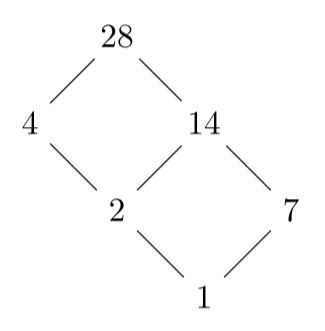
\includegraphics[scale=0.5]{hasse-diagram-1}
    \end{center}

    Die Teilmengenrelation $\subseteq$ auf der Menge $\mathcal{P}(\{a,b,c\})$, als Hasse-Diagramm dargestellt:
    \vspace{-\topsep}
    \begin{center}
        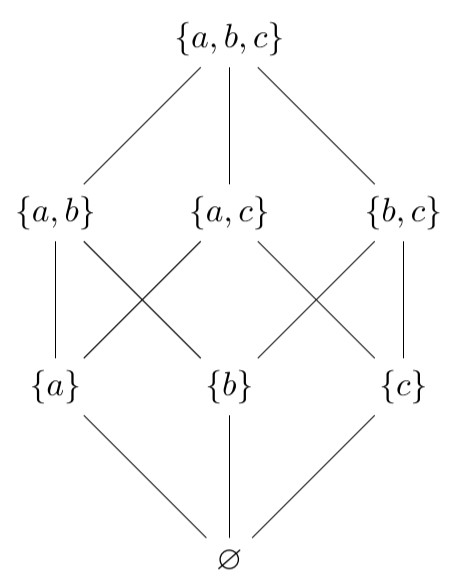
\includegraphics[scale=0.3]{hasse-diagram-2}
    \end{center}
\end{multicols}